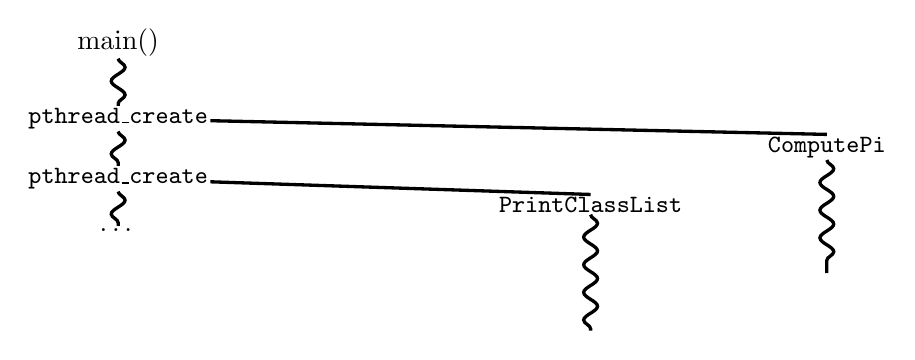
\begin{tikzpicture}
    \tikzset{
        thread/.style={very thick,draw,decorate,decoration=snake},
        split/.style={very thick,draw},
        marker/.style={thin,draw},
        y=0.8cm,
        every node/.style={inner sep=0.1mm}
    }
    \draw[thread] (0, 0) node[above] {main()}-- ++(0, -.75) node[below,font=\tt\small] (create pi) {pthread\_create};
    \draw[thread] (create pi) -- ++(0, -.75) node[below,font=\tt\small] (create list) {pthread\_create};
    \draw[split] (create pi) -- ++(9, -.25) node[below,font=\tt\small] (computepi){ComputePi};
    \draw[thread] (computepi) -- ++(0, -2);
    \draw[thread] (create list) -- ++(0, -.75) node[below] {\ldots};
    \draw[split] (create list) -- ++(6, -.25) node[below,font=\tt\small] (classlist){PrintClassList};
    \draw[thread] (classlist) -- ++(0, -2);
\end{tikzpicture}